% !TEX program = xelatex
% vim:foldmethod=marker:foldmarker=<<<,>>>
\documentclass[compress]{beamer}

%<<< Preamble
\usepackage[english]{babel}
\usepackage{metalogo}
\usepackage{listings}
\usepackage{fontspec}
\usepackage{amsmath, amssymb}
\usepackage{stackrel}
\usepackage{tikz}
\usepackage{svg}
\usepackage{unicode-math}
\usepackage{subcaption}
\usepackage[theme=nord,charsperline=60,linenumbers]{jlcode}

\usetheme{Nord}

\setmainfont{Roboto}
% \setsansfont{DejaVu Serif}
% \setmonofont{CaskaydiaCove Nerd Font Mono}
\setmonofont{JuliaMono}


\makeatletter
\def\verbatim@nolig@list{}
\newcommand\pin{%
\parbox[t]{10pt}{\raisebox{0.2pt}{\usebeamercolor[fg]{mybullet}{$\ast$}}}}
\makeatother

\newcommand{\E}[1]{\ensuremath{E\left\{#1\right\}}}
\newcommand{\norm}[1]{\ensuremath{\lVert#1\rVert}}
\newcommand*{\thead}[1]{\multicolumn{1}{c}{\bfseries #1}}

\newfontfamily\tabulartext[SizeFeatures={Size=6}]{Roboto}


\hypersetup{
    colorlinks=true,
    urlcolor=NordBlue
}

\DeclareMathOperator*{\argmax}{argmax}
\DeclareMathOperator*{\Var}{Var}

\AtBeginDocument{
    \fontsize{8}{12}
    \selectfont

}

\AtBeginSection[]
{
    \begin{frame}[c,noframenumbering,plain]
        \tableofcontents[sectionstyle=show/hide,subsectionstyle=show/show/hide]
    \end{frame}
}


\AtBeginSubsection[]
{
    \begin{frame}[c,noframenumbering,plain]
        \tableofcontents[sectionstyle=show/hide,subsectionstyle=show/shaded/hide]
    \end{frame}
}
%>>>

\title{Project III: Spectral Estimation}
\subtitle{}
\author{\Large Simon Andreas Bjørn}
\date{\large March 14, 2023}

\begin{document}

\begin{frame}[plain,noframenumbering]
    \maketitle
\end{frame}

\begin{frame}[fragile] % <<< Periodogram
    \frametitle{Periodogram}
    \begin{columns}
        \begin{column}{0.5\textwidth}
            Define the periodogram function
            \begin{jllisting}[gobble=16]
                function PSD(x)
                    N = length(x) xₙ = x
                    R = conv(xₙ,conj(xₙ))
                    P = fft(R)
                    return abs.(P).^2
                end
            \end{jllisting}
            And apply it
            \begin{jllisting}[gobble=16]
                N = 1024
                arr = data[1200:1200+N-1, 14]
                Ω = range(-fs/2,fs/2,2N-1)
                Pₓₓ = PSD(arr)./N;
            \end{jllisting}
        \end{column}
        \begin{column}{0.5\textwidth}
            Plotting the PSD of given array yields the following plot
            \begin{figure}
                \includegraphics[width=\columnwidth]{"../1a.pdf"}
            \end{figure}
        \end{column}
    \end{columns}
\end{frame} 
% >>>

\begin{frame}[fragile] % <<< Tempered periodogram
    \frametitle{Tempered periodogram}
    \begin{columns}
        \begin{column}{0.5\textwidth}
            We perform a similar action but include a window on with the array.
            I chose a kaiser window with $\beta = 2.5$. \\
            We also need to normalize with 
            \begin{equation*}
                U = \sum^{N}_{n=1}{\left|W\left(n\right)^2\right|}
            \end{equation*}
            \begin{jllisting}[gobble=16]
                window_func = kaiser(N,2.5);

                U = sum(abs.(window_func).^2)/N
                Pₓₓ2 = PSD(arr.*window_func)./(U*N);
            \end{jllisting}
        \end{column}
        \begin{column}{0.5\textwidth}
            Plotting the PSD yields the following
            \begin{figure}
                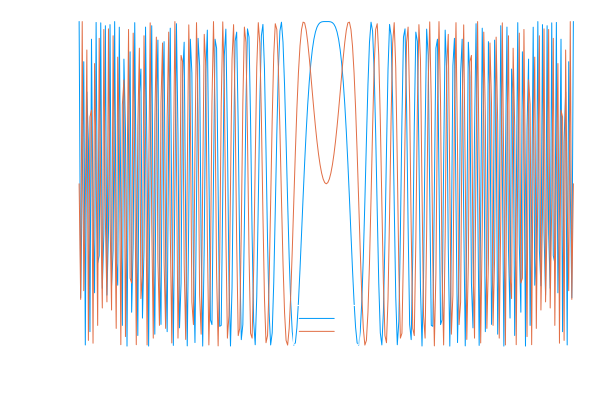
\includegraphics[width=\columnwidth]{"../1b.pdf"}
            \end{figure}
        \end{column}
    \end{columns}
\end{frame}
% >>>

\begin{frame}[fragile] % <<< Periodogram with Welch's method
    \frametitle{Periodogram with Welch's method}
    I implement the wlech method by generating slices of the array
    corresponding to the Welch method's parameters, then mapping the periodogram
    on each array-slice.
    \begin{columns}
        \begin{column}{0.5\textwidth}
            \begin{jllisting}[gobble=16]
                function welch(x, L=256, O = 0.5)
                    N = length(x)
                    D = Int(floor(L*O)) # Overlap 
                    K = (N-L)÷D+1  # Number of slices
                    slices = [a:a+L-1 for a=1:D:K*D]
                    return mapreduce(permutedims, vcat, [x[slice] for slice=slices])
                end

                # Mapping the slices onto the array
                welch_arr = welch(arr)
                K, L = size(welch_arr)
                Uw = sum(abs.(window_func).^2)/N
                window_func = kaiser(L, 2.5)
                Pₓₓw = 1/(Uw*L) * mapslices(
                    PSD ∘ (x->x.*window_func), 
                    welch_arr, 
                    dims=2
                )

                Ωw = range(-fs/2,fs/2,2L-1)
                Pₓₓw = mean(Pₓₓw, dims=1)
            \end{jllisting}
        \end{column}
        \begin{column}{0.5\textwidth}
            \begin{figure}
                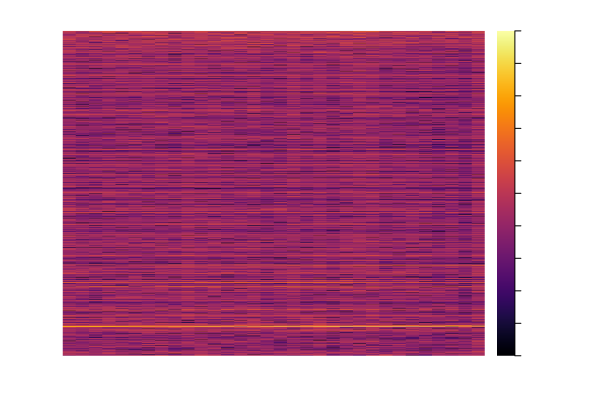
\includegraphics[width=\columnwidth]{"../1c.pdf"}
            \end{figure}
        \end{column}
    \end{columns}
\end{frame}
% >>>

\begin{frame}[fragile] % <<< Periodogram with multitaper
    \frametitle{Periodogram with multitaper}
    \begin{columns}
        \begin{column}{0.5\textwidth}
            The {\texttt pmtm} function does not exist in Julia yet,
            so we do it manually. We define the time-bandwidth product (which i
            set to 2), and we create each of the tapers individually, mapping
            them onto the array, then mapping the periodogram over each. The
            resulting averaged periodogram should be the same.
            \begin{jllisting}[gobble=16]
                nw = 2
                tapers = dpss(N, nw)
                N,K = size(tapers)
                Umt = sum(abs.(tapers).^2, dims=1)/N
                Sxxs = mapslices(PSD, arr.*tapers, dims=1)./(Umt*K)
                Pₓₓmt = mean(Sxxs, dims=2);
            \end{jllisting}
        \end{column}
        \begin{column}{0.5\textwidth}
            Plotting yields
            \begin{figure}
                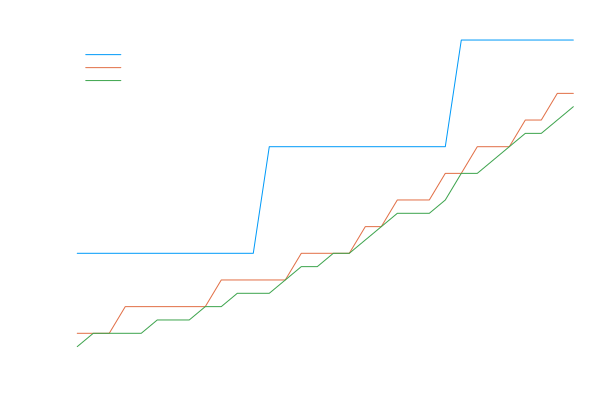
\includegraphics[width=\columnwidth]{"../1d.pdf"}
            \end{figure}
        \end{column}
    \end{columns}
\end{frame}
% >>>

\begin{frame} % <<< Comparing the periodograms
    \frametitle{Comparing the periodograms}
    \begin{columns}
        \begin{column}{0.5\textwidth}
            \begin{figure}
                \includegraphics[width=\columnwidth]{"../1e.pdf"}
            \end{figure}
        \end{column}
        \begin{column}{0.5\textwidth}
            \begin{figure}
                \includegraphics[width=\columnwidth]{"../1f.pdf"}
            \end{figure}
        \end{column}
    \end{columns}
\end{frame} % >>>


\end{document}
